%%%%%%%%%%%%%%%%%%%%%%%%%%%%%%%%%%%%%%%%%
% University/School Laboratory Report
% LaTeX Template
% Version 3.1 (25/3/14)
%
% This template has been downloaded from:
% http://www.LaTeXTemplates.com
%
% Original author:
% Linux and Unix Users Group at Virginia Tech Wiki 
% (https://vtluug.org/wiki/Example_LaTeX_chem_lab_report)
%
% License:
% CC BY-NC-SA 3.0 (http://creativecommons.org/licenses/by-nc-sa/3.0/)
%
%%%%%%%%%%%%%%%%%%%%%%%%%%%%%%%%%%%%%%%%%

\documentclass{article}

%\usepackage[version=3]{mhchem} % Package for chemical equation typesetting
%\usepackage{siunitx} % Provides the \SI{}{} and \si{} command for typesetting SI units
\usepackage{graphicx} % Required for the inclusion of images
\usepackage{natbib} % Required to change bibliography style to APA
\usepackage{amsmath} % Required for some math elements 
\usepackage{listings}
\lstset{basicstyle=\ttfamily\small, breaklines=true}
\setlength\parindent{2pt} % Removes all indentation from paragraphs

%\renewcommand{\labelenumi}{\alph{enumi}.} % Make numbering in the enumerate environment by letter rather than number (e.g. section 6)

%\usepackage{times} % Uncomment to use the Times New Roman font


%----------------------------------------------------------------------------------------
%	DOCUMENT INFORMATION
%----------------------------------------------------------------------------------------

\title{Genetic Algorithm\\MALIS} % Title

\author{Simone \textsc{Rossi}} % Author name

\date{\today} % Date for the report

\begin{document}

\maketitle % Insert the title, author and date

\begin{center}
\begin{tabular}{l r}
Date Performed: & data \\ % Date the experiment was performed
Partners: & Simone Rossi \\ % Partner names
          & Fabian Sperrle\\
%Instructor: & Professor Smith % Instructor/supervisor
\end{tabular}
\end{center}

% If you wish to include an abstract, uncomment the lines below
% \begin{abstract}
% Abstract text
% \end{abstract}

%----------------------------------------------------------------------------------------
%	SECTION 1
%----------------------------------------------------------------------------------------

\section{Chromosome genetic operators}

\textsc{Mutation Test}
\lstinputlisting[firstline=1, lastline=16]{../result/exercise1/exercise1.txt}
\newpage
\textsc{Crossover Test}
\lstinputlisting[firstline=17]{../result/exercise1/exercise1.txt}

\section{Population evolution on a circle}
\lstinputlisting[firstline=1]{../result/exercise2/exercise2.txt}

\begin{figure}[!ht]
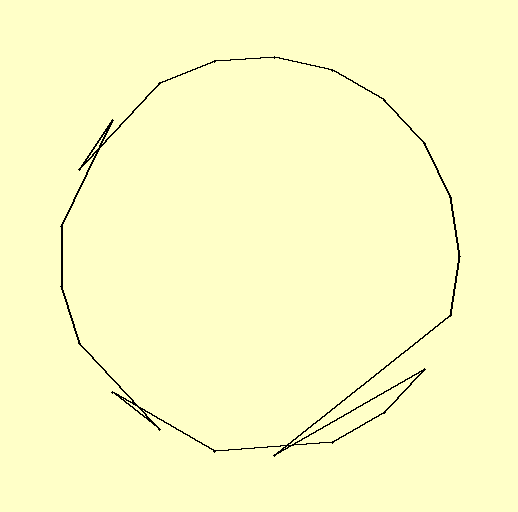
\includegraphics[width=\textwidth]{../result/exercise2/best.png}
\caption{Best result after 96079 generations}
\end{figure}

\newpage
\section{Population evolution on cities in France}
In the next table, we will report the best result out of three runs of every combinations between mutation rate and population size (the complete dump of the experiment can be found in the \texttt{result} directory).

\begin{table}
\centering
\caption{Results using different combinations of mutation rate (columns) and population size (rows)}
\begin{tabular}{c||c|c|c|c}
&10 & 50 & 100 & 500\\
\hline
0.01&1944&1962&2013&1983
\hline
0.1&2076&2159&2117&2144\\
\hline
0.5&2264&2259&2296&2217\\
\hline
\end{tabular}
\end{table}

As result, it seems that the best combination in out case is with a population size of 10 and a mutation rate of 0.01\%. In general, according to these results, increasing the population size doesn't heavly change the final resul; on the contrary, decreasing mutation rate, the overall performance seems to increase.

\begin{figure}
\centering
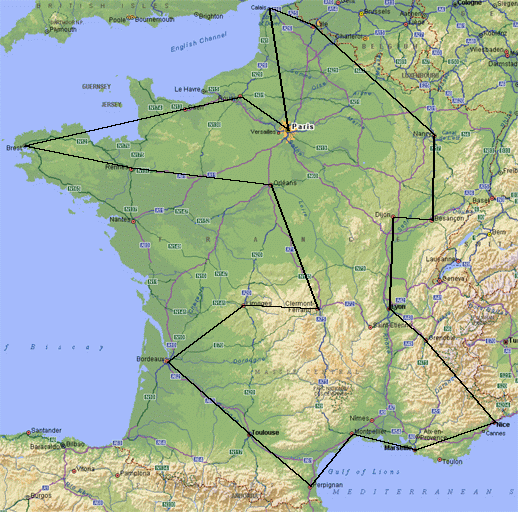
\includegraphics[width=\textwidth]{../result/exercise3/10_1_3/best.png}
\caption{Best result out of 36 different run with 12 different combinations of parameters}
\end{figure}    
\end{document}
